\documentclass[11pt]{article}
\usepackage{CJK}
\usepackage[top=2cm, bottom=2cm, left=2cm, right=2cm]{geometry}
\usepackage{algorithm}
\usepackage{algorithmicx}
\usepackage{algpseudocode}
\usepackage{amsmath}
\usepackage{enumerate}
\usepackage{tikz}

%\floatname{algorithm}{算法}
%\renewcommand{\algorithmicrequire}{\textbf{输入:}}
%\renewcommand{\algorithmicensure}{\textbf{输出:}}
    \title{091M4041H - Assignment 1}
    \author{No. 201628017729008,  Lin Lingfeng}

\begin{document}
\begin{CJK*}{UTF8}{gkai}
    \maketitle

    \section{Problem 1}

    \paragraph{} You are interested in analyzing some hard-to-obtain data from two separate databases. Each database contains $n$ numerical values, so there are $2n$ values total and you may assume that no two values are the same. You'd like to determine the median of this set of $2n$ values, which we will define here to be the $n^{th}$ smallest value.

    \paragraph{}However, the only way you can access these values is through $queries$ to the databases. In a single query, you can specify a value $k$ to one of the two databases, and the chosen database will return the $k^{th}$ smallest value that it contains. Since queries are expensive, you would like to compute the median using as few queries as possible.

    \paragraph{}Give an algorithm that finds the median value using at most $O(\log n)$ queries.

    \paragraph{}\textbf{Solution:}\\
     We call the two separate databases $D_1$, $D_2$.\\
     The median must be between the median of $D_1$ and the median of $D_2$. A divide and conquer approach is designed based on above case. In addition, We can only access database by \emph{queries}, the recursive calls must track the portion of the database is still under consideration.

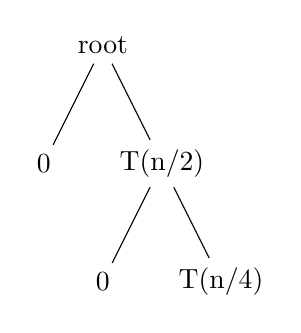
\begin{tikzpicture}
\node {root}
child {node {0}}
child {node {T(n/2)}
child {node {0}}
child {node {T(n/4)}}
};
\end{tikzpicture}


    \paragraph{}\textbf{Algorithm:}\\
    Assume that \textbf{Query(D,k)} is the function to query the $k^{th}$ smallest value that $D$ contains. We run \textbf{FindMedian(D1,1,n,D2,1,n)} to produce the median.
    \begin{algorithm}
        \caption{Find Median in two databases} %{用归并排序求逆序数}
        \begin{algorithmic}[1] %每行显示行号
            \Require $database$: $D_1$, $D_2$, \qquad The size of $D_1$, $D_2$: $n$, $n$
            \Ensure median number
            \Function {Query}{$D,k$}
                \State $result \gets D$
                \If {$size(result) < k$}
                    \State error
                    %\State $middle \gets (left + right) / 2$
                    %\State $result \gets result +$ \Call{MergerSort}{$Array, left, middle$}
                    %\State $result \gets result +$ \Call{MergerSort}{$Array, middle, right$}
                    %\State $result \gets result +$ \Call{Merger}{$Array,left,middle,right$}
                \EndIf
                \State \Return{$result(k)$}
            \EndFunction
            \State

            \Function{FindMedian}{$D_1, lower1, upper1, D_2, lower2, upper2$}
                \State //$k_i$ is a point to specify the median of $D_i$[$lower_i$,...,$upper_i$]
                %\State //$k_2$ is a point to specify the median of $D_2$[$lower_2$,...,$upper_2$]
                \State $k_1\gets lower1+floor((upper1-lower1)/2)$
                \State $k_2\gets lower2+floor((upper2-lower2)/2)$
                \State //$m_i$ get the median of $D_i$[$lower_i$,...,$upper_i$]
                %\State //$m_2$ get the median of $D_2$[$lower_2$,...,$upper_2$]
                \State $m_1\gets Query(D_1,k_1)$
                \State $m_2\gets Query(D_2,k_2)$
                \If{$m_1$ \textgreater $m_2$}
                    \State //finish query and return the median
                    \If{$lower_1$ = $lower_2$ and $upper_1$ = $upper_2$}
                        \State return $m_2$;
                    \State //continue searching in the upper half of $D_2$[$lower_2$,...,$upper_2$] and
                    \State //the lower half of $D_1$[$lower_1$,...,$upper_1$]
                    \Else
                        \State //if($upper_2$ - $lower_2$) is even, then we keep $D[k]$ to make sure that
                        \State //$D_1$[$lower_1$,...,$k_1$] and $D_2$[$k_2$,...,$upper_2$] have the same number of elements.
                        \If{($upper_2$ - $lower_2$) is even}
                            \State return FindMedian($D_1, lower_1, k_1, D_2, k_2, upper_2$)
                        \Else
                        \State //if($upper_2$ - $lower_2$) is odd, then we remove $D[k]$ to make sure that
                        \State //$D_1$[$lower_1$,...,$k_1$] and $D_2$[$k_2+1$,...,$upper_2$] have the same number of elements.
                            \State return FindMedian($D_1, lower_1, k_1, D_2, k_2+1, upper_2$)
                        \EndIf
                    \EndIf
                \Else
                    %\State //finish query and return the median
                    \If{$lower_1$ = $lower_2$ and $upper_1$ = $upper_2$}
                        \State return $m_1$;
                    %\State //continue searching in the lower half of $D_2$[$lower_2$,...,$upper_2$] and
                    %\State //the upper half of $D_1$[$lower_1$,...,$upper_1$]
                    \Else
                        \If{($upper_1$ - $lower_1$) is even}
                            \State return FindMedian($D_1,k_1,upper_1,D_2,lower_1,k_2$)
                        \Else
                            \State return FindMedian($D_1,k_1+1,upper_1,D_2,lower_2,k_2$)
                        \EndIf
                    \EndIf
                \EndIf

            \EndFunction
        \end{algorithmic}
    \end{algorithm}

\paragraph{}\textbf{Correctness Proof:} We prove by induction method.\\
\begin{enumerate}[step 1]
    \item  When $n$ = 1, each database has one element. By execute the algorithm, we return the smaller one of the two elements, which satisfies the definition of median.

    \item  Suppose that the algorithm works correctly for $1,2,...,n-1$, then we will prove that it is also right for $n$.
    \item  For $n$, the median of $D_1$ is $m_1$, and the median of $D_2$ is $m_2$. We prove that the algorithm works correctly for the case that $m_1 \textgreater m_2$ and that $n$ is even. Similar arguments can be applied to the other three cases.\\
        When $m_1 \textgreater m_2$ and $n$ is even, $n-1$ is odd, the algorithm returns $mn$, the median of $D_1[1,...,\frac{n}{n}]$ and $D_2[\frac{n}{2}+1,...,n]$. By the induction hypothesis, we only need to show that $m$ is also the median of $D_1$ and $D_2$.\\
        First, it is easy to see that $m_1 \ge m \ge m_2$. (If $m \textgreater m_1$, then the $n/2$ numbers in $D_1[1,...,\frac{n}{2}]$ will be strictly smaller than $m$, contradicting the definition of median. Hence, $m \le m_1$. Similar arguments can be used to get $m \ge m_2$.) Therefore, by the definition of the median, the numbers in $D_1[\frac{n}{2}+1,...,n]$ are greater than $m$; and the numbers in $D_2[1,...,\frac{n}{2}]$ are smaller than or equal to $m$.\\
        Second, by the induction hypothesis and also by the definition of median, in $D_1[1,...,\frac{n}{2}]$ and $D_2[\frac{n}{2}+1,...,n]$, exactly $\frac{n}{2}$ numbers are greater than $m$; and exactly $\frac{n}{2}$ numbers are greater than $m$.\\
        In total, there are $n$ numbers in $D_1$ and $D_2$ that are smaller than or equal to $m$, and there are $n$ numbers in $D_1$ and $D_2$ that are greater than $m$, meaning that $m$ is indeed the median for $D_1$ and $D_2$.
\end{enumerate}

\paragraph{}\textbf{Runtime Analysis:} The algorithm is a divide and conquer approach. Each time, there is only one subproblem, the size of the problem is reduced by half (each database is kept only half of its elements), and two queries (issue one query to each database) are sent to the databases. Hence, the recurrence relation is $T(n) = T(n/2)+2$. Thus, $T(n) = O(\log{n})$.

\section{Problem 2}

\paragraph{}Find the $k^{th}$ largest element in an unsorted array. Note that it is the $k$th largest element in the sorted order, not the $k^{th}$ distinct element.

\paragraph{}INPUT: An unsorted array $A$ and $k$.

\paragraph{}OUTPUT: The $k^{th}$ largest element in the unsorted array $A$.

    \paragraph{}\textbf{Solution:}\\
    We can first order the array $A$ then query the $k^{th}$ largest element.
    Quicksort is a divide-and-conquer sorting algorithm in which division is dynamically carried out (as opposed to static division in Mergesort).\\
    Divide: Rearrange the elements and split the array into two subarrays and an element in between such that so that each element in the left subarray is less than or equal the middle element and each element in the right subarray is greater than the middle element.\\
    Conquer: Recursively sort the two subarrays.


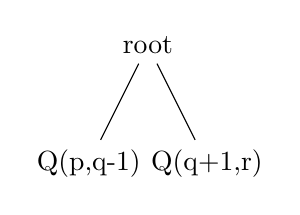
\begin{tikzpicture}
\node {root}
child {node {Q(p,q-1)}}
child {node {Q(q+1,r)}
};
\end{tikzpicture}


    \paragraph{}\textbf{Algorithm:}\\
    Assume that \textbf{QuickSort(A,1,n)} is the function to order the array $A$. Function \textbf{Partition} is to determine the pivot.
    \begin{algorithm}
        \caption{QuickSortFor $ k^{th} $ LargestElement}
        \begin{algorithmic}[1] %每行显示行号
            \Require $database$: $A$, \qquad The size of $A$: $n$
            \Ensure $ k^{th} $ largest element
            \Function {QuickSort}{$A,n$}
                \State QuickSort'($A,1,n$)
                \vspace{3mm}
                \State QuickSort'($A,1,n$)
                \If {$p > k$}
                    \State $q \gets Partition(A,p,r)$
                \EndIf
                \State QuickSort'($A,p,q-1$)
                \State QuickSort'($A,q+1,r$)
                %\State \Return{$result(k)$}
            \EndFunction
            \State

            \Function{Partition}{$A,p,r$}
                \State x = A[r]
                \State $i\gets p-1$
                \State $j\gets p$
                \For{\texttt{$j < r-1 p$}}
                    \If{$A[j] \leq x$}
                        \State $i \gets i+1$
                        \State Exchange A[i] and A[j]
                    \Else
                    \EndIf
                    \State Exchange A[i+1] and A[r]
                \EndFor
                \State return i+1
            \EndFunction
        \end{algorithmic}
    \end{algorithm}

\paragraph{}\textbf{Correctness Proof:}
    Let $(A,p,r)$ be any input to \textbf{Partition} and let $q$ be the output of \textbf{Partition} on this input. Suppose $1 \leq p < r$. Let x=A[r]. We will
prove the correctness using loop invariant. The loop invariant we use is: at the beginning of the for-loop, for all $k$, $p \leq k < r$, the following properties hold:

\begin{enumerate}[ 1]
    \item  If $p \leq k <i$, then $A[k] \leq x$.

    \item  If $i+1 \leq k <j-1$, then $A[k] \textgreater x$.
    \item  If $k = r$, then $A[k]=x$.
\end{enumerate}


\paragraph{}\textbf{Runtime Analysis:} \\
Let T be the worst-case running time of Quicksort. Then T(n) = T(1) + T(n-1) + $O(n)$, thus T(n) = $O(n^2)$.\\
The best cases are when the array is split half and half. Then each element belongs to a region in which \textbf{Partition} is carried out at most $\lceil log{n} \rceil$ times, so it's O(n{log{n)}}.


\section{Problem 3}

\paragraph{}Consider an $n$-node complete binary tree $T$, where $n=2^d-1$ for some $d$. Each node $v$ of $T$ is labeled with a real number $x_v$. You may assume that the real numbers labeling the nodes are all distinct. A node $v$ of $T$ is a $local\ minimum$ if the label $x_v$ is less than the label $x_w$ for all nodes $w$ that are joined to $v$ by an edge.

\paragraph{}You are given such a complete binary tree $T$, but the labeling is only specified in the following $implicit$ way: for each node $v$, you can determine the value $x_v$ by $probing$ the node $v$. Show how to find a local minimum of $T$ using only $O(\log n)\ probes$ to the nodes of $T$.


    \paragraph{}\textbf{Solution:}\\
    In this problem, we define probe() to get the value of one node. We recursively find the smallest one in its children and itself. If itself has the smallest value, then we return its value or we recursively compare the smallest child and its subtree,


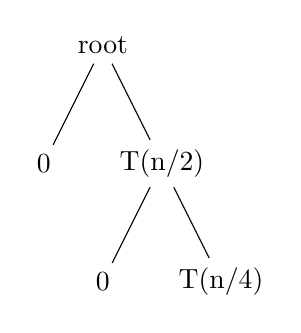
\begin{tikzpicture}
\node {root}
child {node {0}}
child {node {T(n/2)}
child {node {0}}
child {node {T(n/4)}}
};
\end{tikzpicture}

    \paragraph{}\textbf{Algorithm:}\\
        \begin{algorithm}
        \caption{FindMin}
        \begin{algorithmic}[1]
            \Require $database$: $T$, \qquad The size of $T$: $n$
            \Ensure smallest one
            \Function {FindMin}{$T$}
                \If {min(prode(T.left()), probe(T.right()), probe(T.root())) ==probe(T.root())}
                    \State return T.root()
                \Else
                    \If{probe(T.left())$>$ probe(T.right()) }
                        \State FindMin($T.right()$)
                    \Else
                        \State FindMin($T.left()$)
                    \EndIf
                \EndIf
            \EndFunction
            \State
        \end{algorithmic}
    \end{algorithm}


\paragraph{}\textbf{Correctness Proof:}

\begin{enumerate}[ 1]
    \item  Initialization. At first step, the initial node we input is the root, we compare the value of and it and its two children. The node we may return is the smallest of them.

    \item  Maintenance. Suppose the right child is smallest, we compare the value of this new node and its children, this process recursively goes forward until one node whose root has the smallest value.
    \item  Termination. At termination, since the root's value is smallest, the local minimum is found and it is the smallest in the path through.
\end{enumerate}


\paragraph{}\textbf{Runtime Analysis:} \\
 T(n) = T(n/2) + $O(n)$, thus T(n) = $O(logn)$.



%\section{Problem 8}
%
%\paragraph{}The attached file Q8.txt contains 100,000 integers between 1 and 100,000 (each row has a single integer), the order of these integers is random and no integer is repeated.
%\begin{enumerate}
% \item Write a program to implement the Sort-and-Count algorithms in your favorite language, find the number of inversions in the given file.
% \item In the lecture, we count the number of inversions in $O(n \log n)$ time, using the Merge-Sort idea. Is it possible to use the Quick-Sort idea instead ? \\
%If possible, implement the algorithm in your favourite language, run it over the given file, and compare its running time with the one above.
%If not, give a explanation.
%\end{enumerate}
%
%\section{Problem 9}
%
%\paragraph{}Implement the algorithm for the closest pair problem in your favourite language.
%
%\paragraph{} INPUT: $n$ points in a plane.
%
%\paragraph{} OUTPUT: The pair with the least Euclidean distance.
%
%    \paragraph{}\textbf{Solution:}\\
%    For the $n$ points set, we divide it into two subsets. Finding the closest pairs in each half. With the observation that the closest pair is located in left half, or right half, or within $\sigma$ of the middle line L.
%
%    \paragraph{}\textbf{Algorithm:}\\



\end{CJK*}
\end{document} 
